\chapter{Analyse}

\section{Ist-Situation}

In der Vorgängerarbeit \enquote{Cygnet} von Stefan Rohner und Marco
Tanner\cite{cygnet:2013} wurde der Policy Manager \enquote{strongTNC}
implementiert. Das Produkt und die Codebasis dienen als Grundlage
für diese Arbeit.

Im Bereich des SWID Generators gibt es zur Zeit noch keine bestehenden Produkte.

\subsection{Elemente der strongTNC App}
Im Folgenden werden die zentralen Elemente der strongTNC Umgebung beschrieben.
Die Namen entsprechen jenen der bestehenden Django-Models. Diese Liste soll einen
kurzen Überblick geben, eine ausführliche Beschreibung ist in der Dokumentation
\enquote{Cygnet}\cite{cygnet:2013} zu finden.

\begin{description}
	\item[Policy] Eine Policy beschreibt eine zu überprüfende Richtlinie. Durch
	einen Policytyp wird festgelegt, was überprüft werden soll (z.B erlaubte offene
	Ports, installierte Software). Weiterhin kann festgelegt werden, welche Aktion
	bei positivem oder negativen Ausgang der Messung (überprüfen der Richtlinie)
	ausgeführt werden soll.
	
	\item[Enforcement] Policies werden durch Enforcements erzwungen. Ein
	Enforcement wird einer Gruppe von Geräten zugeteilt. Spezifiert wird zudem in
	welchen zeitlichen Abständen die verknüpfe Policy überprüft wird.

	\item[Group] Geräte können in Gruppen zusammengefasst werden. Gruppen dienen
	letztendlich dazu, zu bestimmen, welche Enforcements zur Anwendung kommen.
	Gruppen lassen sich hierarchisch aufbauen.

	\item[Session] Wenn sich ein Gerät mit einem strongSwan TNC Netzwerk verbindet,
	wird durch strongSwan eine Session für das verbundene Gerät erstellt. Sämtliche
	Messungen werden mit einer Session verknüpft.

	\item[Workitem] Für jede Policy, die durch ein Enforcement während einer
	Session geprüft werden muss, wird ein Workitem erstellt. Diese Workitems werden
	durch die IMVs (Integrity Measurement Validator) von strongSwan abgearbeitet.
	Die Resultate werden nach den Messungen in den Workitems abgelegt.

	\item[Device] Ein Device repräsentiert ein Gerät, welches sich in ein
	strongSwan TNC Netzwerk verbinden kann. Ein Gerät wird durch die Kombination
	einer eindeutigen Hardware ID, sowie dem Betriebssystem (siehe Product)
	identifiziert. Ein Device ist Mitglied einer oder mehrerer Gruppen, diese
	Mitgliedschaft bestimmt welche Policies auf das Gerät angewendet werden.

	\item[Product] Ein Product entspricht dem Betriebssystem eines Devices. Einem
	Product können Gruppen zugeteilt werden, welche auf Devices mit
	diesem Product übertragen werden. Diese Gruppen stellen insofern die
	Standardgruppen eines Gerätes mit einem bestimmten Betriebssystem dar.

	\item[Package] Ein Package beschreibt ein Softwarepaket. Packages werden mit
	Versionen verknüpft.

	\item[Version] Eine Version ist immer mit einem Package und einem Product
	verknüpft. Das heisst, für jedes Betriebssystem existiert eine eigene Version,
	auch wenn die Versionsbezeichnung dieselbe ist. Versionen können global als
	\enquote{blacklisted} und \enquote{Security patch} markiert werden. Versionen
	können Messobjekte einer Policy sein.

	\item[Directory] Ein Directory kann Bestandteil einer Policy und somit
	Grundlage einer Messung sein.

	\item[File] Files dienen als Grundlage für File-Messungen.

	\item[FileHash] Bei File-Messungen können Hashes einer gewissen Datei erfasst
	werden, diese werden zusammen mit dem Product des gemessenen Gerätes einem
	File zugewiesen.
	
\end{description}

In \autoref{django-ist-diagram} ist eine Übersicht der verwendeten Django-Models
zu sehen:
\begin{figure}[H]
	\centering
	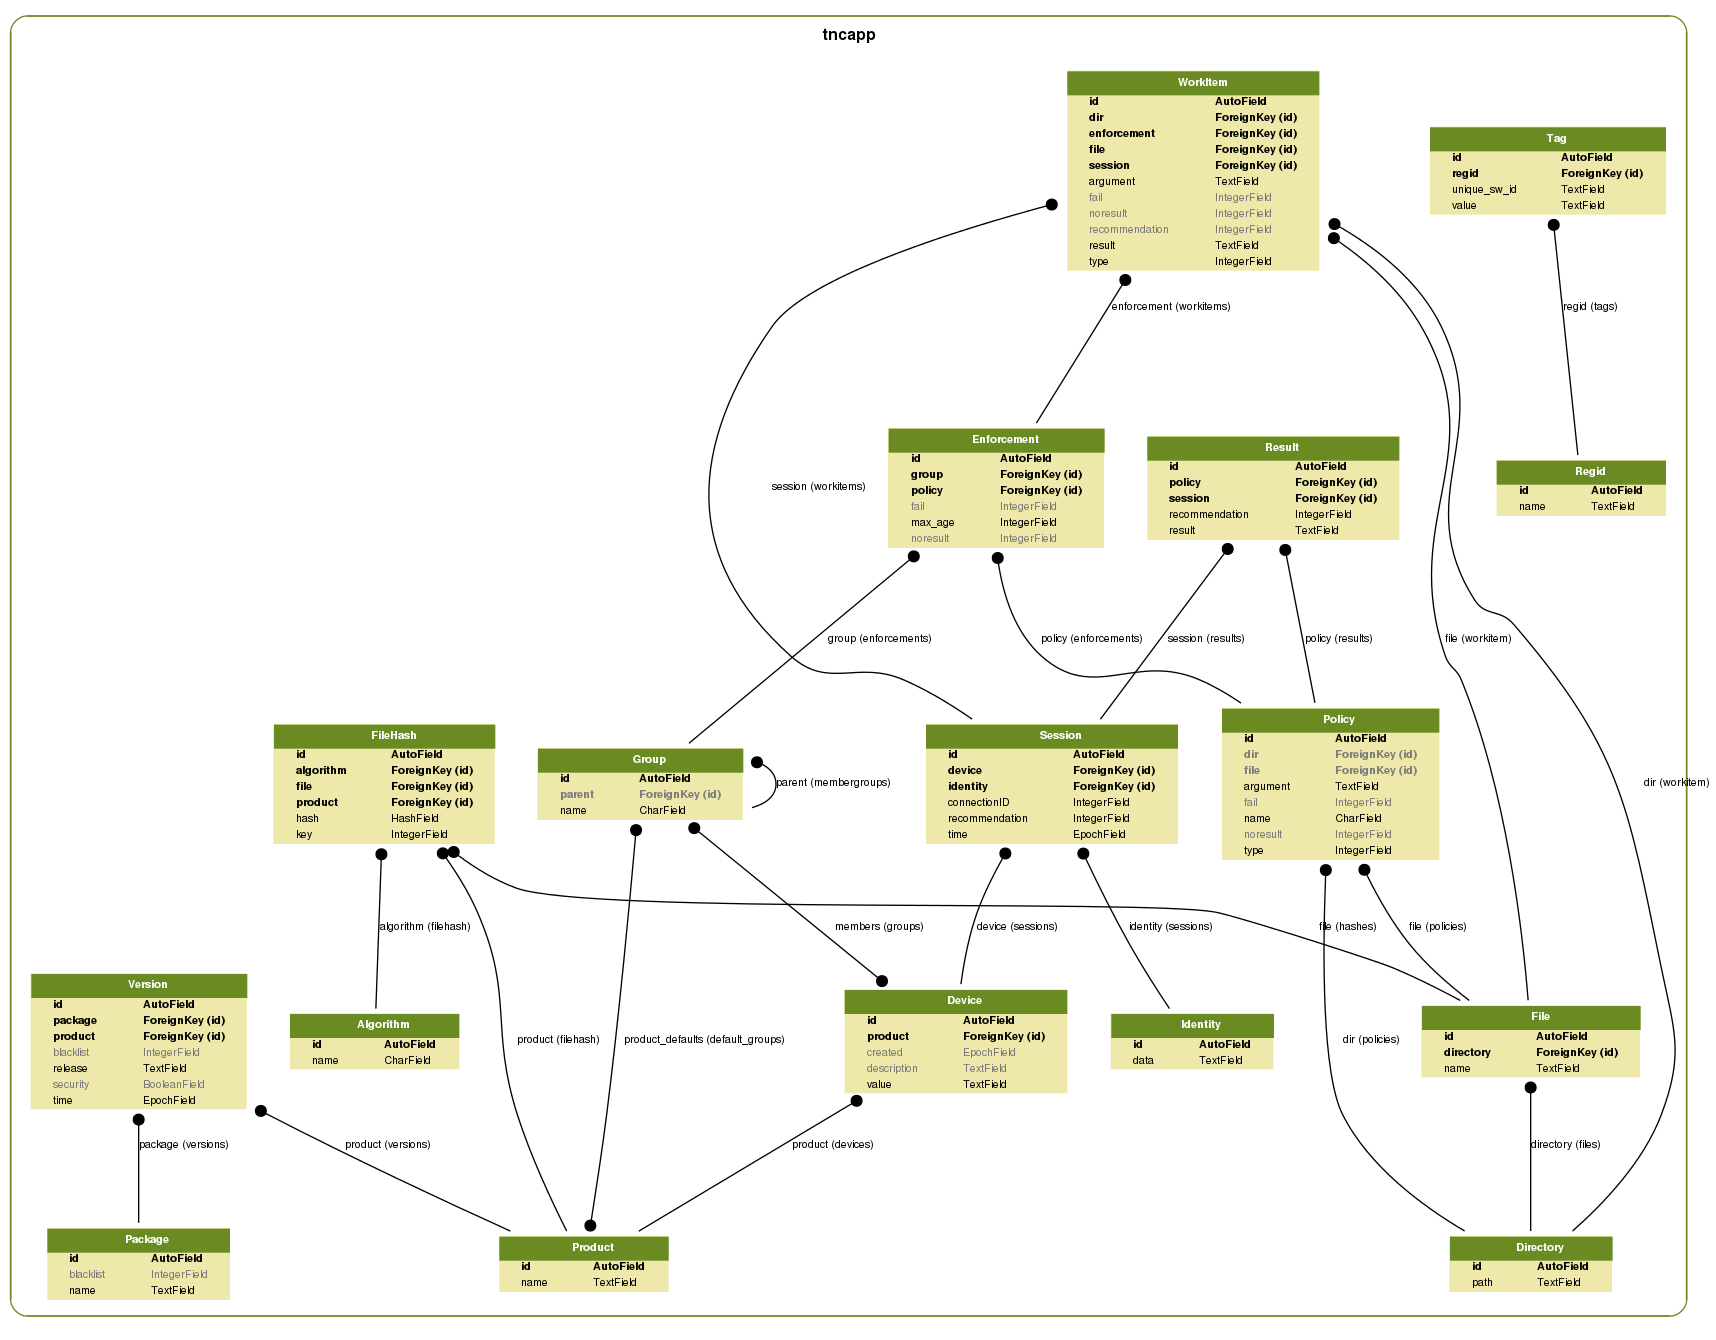
\includegraphics[width=\textwidth]{images/architecture/django_apps_ist}
	\caption{Monolithische Django App}
	\label{django-ist-diagram}
\end{figure}

\subsection{Ablauf einer TNC Messung mit strongSwan und strongTNC}
Wenn sich ein Gerät in ein strongSwan TNC Netzwerk verbindet, wird durch einen
IMV eine strongTNC Session gestartet, darauf wird das Gerät anhand seiner
Hardware ID und des Betriebssystems identifiziert. Falls sich das Gerät zum
ersten mal verbindet, wird es neu erfasst. Anhand der Gruppen denen das Gerät
angehört werden die relevanten Enforcements gesammelt und daraus Workitems
generiert. Diese Vorgänge werden derzeit alle durch den IMV durch direkten
Zugriff auf die Datenbank durchgeführt.\\
Die Workitems werden abgeholt und durch strongSwan verwaltet. Verschiedene IMV
führen dann die Messungen, anhand der Workitems durch. Die Ergebnisse der
Messungen werden durch die IMVs in die Workitems der strongTNC Datenbank
geschrieben. Wenn die Workitems abgearbeitet sind wird die Session
abgeschlossen. Ein IMV schliesst die Session in der strongTNC Datenbank ab, die
Resultate der Workitems werden in archiviert.\\
Anhand der einzelnen Resultate der Workitems fällt der TNC Server nun eine
abschliessende Entscheidung daüber, ob das Gerät in das Netzwerk zugelassen wird
oder nicht.

Den Ablauf einer Messung kann man dem folgenden Sequenzdiagramm,
\autoref{masurement-diagramm}, entnehmen:
\begin{figure}[H]	
	\centering
	\begin{tikzpicture}
	\begin{umlseqdiag}

		% Objekte
		\umlobject{TNC Server}
		\umlobject{IMV Manager}
		\umlmulti{IMVs}
		\umlobject{strongTNC}
		
		% Calls
		\begin{umlcall}[dt=5, op=startSession]
			{TNC Server}{IMV Manager}
		\end{umlcall}
		
		\begin{umlcall}[dt=5, op=startSession]
			{IMV Manager}{IMVs}
		\end{umlcall}	
		
		\begin{umlcall}[dt=5, op=startSession]
			{IMVs}{strongTNC}
		\end{umlcall}
		
		\begin{umlcall}[dt=5, op=evaluateEnforcements]
			{IMVs}{strongTNC}
		\end{umlcall}
		
		\begin{umlcall}[dt=5, op=generateWorkitems]
			{IMVs}{strongTNC}
		\end{umlcall}
		
		\begin{umlcall}[dt=5, op=setWorkitemList]
			{IMVs}{IMV Manager}
		\end{umlcall}	
		
		\begin{umlfragment}[type=loop, label={foreach Workitem}, inner xsep=15, inner ysep=2]
			\begin{umlcall}[dt=9, op=getOpenWorkitem]
				{IMVs}{IMV Manager}
			\end{umlcall}	
			
			\begin{umlcallself}[dt=5, op=doMeasurement]
				{IMVs}
			\end{umlcallself}	
			
			\begin{umlcall}[dt=5, op=storeResult]
				{IMVs}{strongTNC}
			\end{umlcall}
			
		\end{umlfragment}

		\begin{umlcall}[dt=25, op=noWorkitemsLeft]
			{IMV Manager}{TNC Server}
		\end{umlcall}			
		
		\begin{umlcall}[dt=5, op=stopSession]
			{TNC Server}{IMV Manager}
		\end{umlcall}
		
		\begin{umlcall}[dt=5, op=stopSession]
			{IMV Manager}{IMVs}
		\end{umlcall}	
		
		\begin{umlcall}[dt=5, op=stopSession]
			{IMVs}{strongTNC}
		\end{umlcall}
		
		\begin{umlcall}[dt=5, op=cleanUpWorkitems]
			{IMVs}{strongTNC}
		\end{umlcall}

	\end{umlseqdiag}
\end{tikzpicture}

	\caption{Sequenzdiagramm, strongSwan TNC Messung}
	\label{masurement-diagramm}
\end{figure}


\subsection{Stand der strongTNC Webapplikation} 
\label{analyse:stand}

strongTNC ist eine Implementierung eines TNC Policy Managers. Umgesetzt wurde
dieser als Webapp mit dem Python basierten \textit{Django Web Framework} in
Version 1.5\footnote{\url{https://www.djangoproject.com/}}. Die Applikation
bietet Unterstützung für das Verwalten von Geräten, Policies und Enforcements
und erlaubt die Ausführung von Enforcements mittels hierarchischer Gruppen
zu steuern. Stammdaten wie Dateien oder Softwarepakete können eingesehen und
teilweise bearbeitet werden. Auch Messresultate werden passend aufbereitet.

Für SWID Tags besteht derzeit keine Unterstützung. Es wurden zwar bereits Views
für SWID Tags und Regids erstellt, diese haben jedoch ausser der Auflistung der
Datenbankinhalte keine weitere Funktionalität und dienen bisher als Vorschau
für zukünftige Features.

Im Frontend der Webapplikation wurden Bootstrap
2.3\footnote{\url{http://getbootstrap.com/2.3.2/}} sowie jQuery
1.9\footnote{\url{http://jquery.com/1.9}} eingesetzt. Grundsätzlich werden die
Views als \enquote{Master-Detail Ansichten} dargestellt. Als Schnittstelle zur
strongSwan TNC Server Infrastruktur dient eine gemeinsam genutzte
SQLite\footnote{\url{http://www.sqlite.org/}} Datenbank.

Der Code ist in einer einzelnen Django-App organisiert, es gibt keine
thematische Aufteilung in mehrere Apps.

Das Schema der Datenbank ist unabhängig von den Models, diese bilden das
aktuelle Schema ab. Um die Datenbank zu initialisieren wird ein separat
bereitgestelltes SQL Schema verwendet.

Laut dem Technischen Bericht der Vorgängerarbeit
\enquote{Cygnet}\cite{cygnet:2013} sollen die Richtlinien des \enquote{Style
Guide for Python Code}\cite{PEP8:2001}, genannt PEP8, eingehalten werden. Es
existieren elf Unit-Tests, welche den bestehenden Python Code zu 21\% abdecken.


\subsubsection{Einschätzung der Ist-Situation}
\label{analyse:einschaezung}

\begin{description}

\item[SWID Integration] Es existiert noch keine Möglichkeit zur Erfassung und
	Verwaltung von SWID Tags. Die bestehenden Views können gegebenenfalls als
	Vorlage für eine solche Integration verwendet werden.
	
\item[Schnittstelle] Das Verwenden einer gemeinsamen Datenbank stellt in unseren
	Augen ein Architekturproblem dar, welches dringend angegangen werden muss.
	Einerseits wird die Interoperabilität mit anderen Systemen stark
	eingeschränkt, andererseits wird die Wartbarkeit und Ausbaufähigkeit aller
	beteiligten Komponenten erschwert oder verunmöglicht. In diesem Fall wird
	ausserdem SQLite als Datenbank verwendet. SQLite ist nur bei lesendem Zugriff
	mehrbenutzerfähig, bei schreibendem Zugriff wird die Datenbank gesperrt. Da
	eine gemeinsam genutzte Datenbank Mehrbenutzerbetrieb impliziert, besteht in
	diesem Bereich Handlungsbedarf.

\item[Benutzerschnittstelle] Die Benutzeroberfläche wurde noch nicht für den
	Umgang mit grossen Datenmengen optimiert. Es gibt keinen Paging Mechanismus,
	der ein stückweises Ausliefern von Daten oder ein Filtern einer grossen Anzahl
	Objekte erlaubt. Beispielsweise kann das Inventar der Dateinamen in einem
	Linux System durchaus 40000 Objekte umfassen. Wird die vorhandene File View
	aufgerufen, werden alle 40000 Einträge angezeigt.\\ Diesen Datenmengen wird
	zur Zeit noch nicht Rechnung getragen und die aktuelle Oberfläche hat sich
	bereits beim Entwickeln in einer kleinen Umgebung als nicht mehr überschaubar
	erwiesen. Tendentiell ist der Einsatz einer Endpoint Compliance Lösung in
	mittelgrossen und grossen Unternehmungen zu erwarten, dementsprechend ist auch
	die Menge der zu verwaltenden Daten als hoch einzuschätzen.

\item[Django-Apps] Django Webapplikationen lassen sich in Module, sogenannte
	\enquote{Apps}, aufteilen. Diese Möglichkeit wird allerdings bisher nicht
	genutzt. Stattdessen befindet sich der gesamte Code in einer einzelnen App
	namens \texttt{tncapp}. Eine solche Unterteilung würde die Wartbarkeit
	erhöhen.

\item[Datenbank-Schema] Bei der Umsetzung von Webapplikationen mit Django ist es
	gängig, dass das Datenbankschema aus den Models generiert wird. Dadurch muss
	man sich als Entwickler nicht um Schema-Detailfragen kümmern, sondern kann
	sich auf die abstrakten Models konzentrieren. Ein weiterer 
	Vorteil ist, dass das genutzte DBMS beliebig austauschbar ist. Da
	die Datenbank bei strongTNC jedoch als Schnittstelle dient und nicht
	ausschliesslich von Django verwendet wird, kann dieses Feature derzeit nicht
	genutzt werden. Stattdessen bilden die Model-Definitionen den jeweiligen Stand
	der Datenbank (siehe \autoref{fig:database-model}) ab. Weil die Datenbank
	nicht aus den Models generiert wird, ist es möglich, dass die Models und das
	effektive Schema bei Änderungen nicht mehr synchron sind und manuell angepasst
	werden müssen. Eine zentrale \enquote{Autorität} für das Schema sowie die
	Nutzung eines Schema-Migrations-Frameworks würde diese Situation stark
	verbessern.

\item[Codequalität] Obwohl sich die Vorgängerarbeit gemäss eigener Aussagen auf
	die Einhaltung der PEP8-Coderichtlinien\cite{PEP8:2001} beruft
	\cite[S.~79]{cygnet:2013}, wurden diese Richtlinien nicht konsequent
	eingehalten. \\
	Alle Views wurden als Funktionen definiert, obwohl sie häufig über gemeinsame
	Funktionalität verfügen. Auch die zyklomatische Komplexität der Views ist
	oft hoch. Ein klassenbasierter Ansatz, eventuell auch in Kombination
	mit den mitgelieferten generischen Views von Django, könnte die
	Wartbarkeit verbessern. \\
	Die Validierung von übermittelten Formulardaten wurde \enquote{von Hand}
	gemacht, anstatt das vorhandene Formular-Framework von Django zu verwenden. Auch dies
	verursacht mehrfach vorhandenen Code und verletzt unnötigerweise das
	DRY-Prinzip\cite[S.~26--27]{hunt1999pragmatic}. \\
	Statische Code-Analyse zeigt viele Mängel auf, wie beispielsweise
	unerreichbarer Code, ungenutzte Variablen, mehrfach definierte Funktionen oder
	verdeckte Python-Standardfunktionen. \\
	Die Templates sind inkonsistent eingerückt, man findet sich im Markup sehr
	schwer zurecht. Zudem sind sehr viele Elemente -- wie \zb das Suchfeld --
	mehrfach vorhanden und sollten in ein eigenes Include-Template extrahiert
	werden.

\end{description}

\section{Soll-Situation}
\label{analyse:soll-situation}

Nebst den geforderten Pflichtteilen, der Implementation eines SWID Generators
für Linux Systeme und der Integration der SWID Erweiterung in strongTNC,
schlagen wir nachfolgende Anpassungen vor, die wir bei vorhandener Kapazität
noch umsetzen möchten.

\subsection{Entkopplung der Datenbank}
\label{analyse:architekturen}
Wie bereits erwähnt entstehen durch die gemeinsame Nutzung einer SQLite
Datenbank einige Probleme. Nachfolgend möchten wir kurz auf die daraus
resultierenden Nachteile eingehen.

\begin{description}
	\item[Mehrbenutzerfähigkeit] Die Daten einer SQLite Datenbank können nur von
	einem Prozess gleichzeitig geändert werden. Da es sich bei der aktuellen
	Situation aber bereits um eine Multiprozessumgebung handelt ist dieser Einsatz
	denkbar schlecht, und kann zu unerwünschten Locks führen.

	\item[Verteilung der Komponenten] Die Policy Decision Komponente (TNC Server
	aus strongSwan Projekt) kann derzeit nicht getrennt von der strongTNC Webserver
	Komponente betrieben werden. Dies kann in einem Enterprise Deployment
	durchaus erwünscht sein. Beispielsweise der Einsatz eines Windows Webservers
	mit der strongTNC App, während der Enforcement Point auf einem Linux System
	läuft. Zusätzlich kann es aus netzwerktechnischen Gründen bedingt sein, im
	Internet exponierte Komponenten, in diesem Fall den strongSwan VPN Gateway und
	einen Webserver, in getrennten Netzwerksegmenten zu halten. Oder zur
	Lastverteilung auf unterschiedliche Hosts zu verteilen.

	\item[Anbindung an Drittsysteme] Die Anbindung an Umsysteme gestaltet sich als
	kaum realisierbar. Das TNC Framework sieht aber bereits weitere Komponenten,
	wie beispielsweise IF-MAP Devices vor, die integriert werden könnten. Auch eine
	Integration in bestehende Geschäftsprozesse (zum Beispiel CMDB) ist nur schwer realisierbar.
	
	\item[Flexiblere Arbeit mit Django] Wenn die strongTNC Anwendung ihre Datenbank
	nicht mit anderen Systemen teilen muss, können alle
	Datenbank-Abstraktionsfeatures von Django voll ausgenutzt werden. Im Moment muss man sich aktiv um das Datenbankschema kümmern. Dies hätte zur Folge, dass
	auch
	\enquote{Migrations}\footnote{\url{https://docs.djangoproject.com/en/dev/topics/migrations/}} zu verwenden, welche es erlauben Änderungen an den Models automatisiert in die Datenbank einfliessen zu lassen.
	
\end{description} 


\section{Abgrenzung}
Folgende Punkte werden von uns als gegeben betrachtet und sind nicht zentraler
Bestandteil unserer Arbeit:

\begin{description}
	\item[Datenbankschema] Das Schema wird nicht grundlegend geändert, sondern
	übernommen wie es ist. Da verschiedene Komponenten auf die Datenbank zugreifen,
	kann eine Änderung am Schema im schlechtesten Fall eine Anpassung in allen
	Komponenten mit Datenbankzugriff zur Folge haben.

	\item[Benutzerschnittstelle] Das Frontend der Webapp wird nicht grundlegend
	verändert, es werden Korrekturen, Ergänzungen und Anpassungen vorgenommen,
	jedoch ohne dabei das bestehende Layout grundsätzlich zu ändern.

	\item[strongSwan] Anpassungen und Ergänzungen seitens strongSwan sind nicht
	Bestandteil dieser Arbeit. Änderungen in strongTNC, welche Einfluss auf
	strongSwan haben, werden mit den verantwortlichen strongSwan Entwicklern
	besprochen.
\end{description}

\section{ISO Standard 19770-2}
\label{analyse:swidstandard} 
Der ISO Standard 19770-2:2014 ist der zweite Teil einer Gruppe von ISO Standards
zu den Prozessen und Technologien des Software Asset Management. Dieser Teil des
Standards beschreibt den Aufbau und die Verwendung von Software Identification
Tags und befindet sich zur Zeit noch im Entwurfsstadium (\enquote{Draft}).

\subsection{Bestandteile eines SWID Tags}
Nachfolgend eine Zusammenstellung der Bestandteile eines SWID Tags, wie sie in
diesem Projekt verwendet werden. Der Standard beschreibt noch weitere Elemente
und Anwendungsmöglichkeiten, welche in dieser Arbeit allerdings nicht verwendet
werden. Die jeweiligen Listen der Attribute sind nicht vollständig, sondern eine
Auswahl, wie sie für diese Arbeit relevant sind. (ISO
19770-2\cite{iso19770-2}, Seite 19, 8.6)

\begin{description}
	\item[SoftwareIdentity] Repräsentation des Wurzelelementes eines SWID Tags.
	Dieses Element hat Attribute, welche die Anwendung des Tags und dessen Identität,
	innerhalb seiner Entität, beschreiben.
	\begin{description}
		\item[delta] Das \texttt{delta} Attribut beschreibt, ob es sich um ein Patch
		oder eine Modifikation der Software handelt. Dieses Attribut wird von uns
		nicht verwendet, da bei Linux Systemen üblicherweise keine Patches verteilt
		werden, sondern gepatchte Softwarepakete. Der Standardwert ist \texttt{false}.

		\item[name] Dieses Pflichtfeld enthält den Namen der Software so wie man
		üblicherweise darauf verweisen würde.
		
		\item[uniqueId] Die \texttt{uniqueId} ist eine Kennung, die eine Software
		innerhalb des Namespaces des Tag Creators eindeutig identifizieren kann.
		Vorschläge für den Aufbau einer \texttt{uniqueId} sind \texttt{publisher +
		product + version} oder eine GUID. Die \texttt{uniqueId} ist optional.
		
		\item[version] In diesem Attribut wird die Version der Software festgelegt.
		Das Attribut ist optional und hat einen Standardwert von \texttt{0.0}.
	\end{description}
	
	\item[Entity] Beschreibt die Organisation, die für diesen SWID Tag
	verantwortlich ist. In einem Tag können theoretisch beliebig viele Entity
	Elemente enthalten sein. Eine Entity mit der Rolle \texttt{tagcreator} (siehe
	Attribut \texttt{role}) ist obligatorisch. Jeder Tag muss mindestens eine
	Entity mit der Rolle \texttt{tagcreator} enthalten. Das \texttt{Entity} Element
	ist ein Kind des \texttt{SoftwareIdentity} Elements.
	\begin{description}
		\item[name] Name der Organisation, die eine bestimmte Rolle in diesem Tag für
		sich beansprucht. Dieses Attribut ist ein Pflichtfeld.
		
		\item[regid] Die \texttt{regid} ist die \enquote{Unique registration ID} einer
		Organisation. Die \texttt{regid} ist grundsätzlich wie folgt aufgebaut:
		\texttt{regid.YYYY-MM.<reverse domain name>}, die vierstellige Jahreszahl und
		der zweistellige Monat ist das Registrierungsdatum der Domain. Für den Aufbau
		einer \texttt{regid} gibt der Standard noch weitere Richtlinien vor, es ist
		auch definiert wie eine \texttt{regid} für Organisationen ohne registrierte
		Domain auzusehen hat. Dieses Attribut ist optional und wird mit dem
		Standardwert \texttt{invalid.unavailable} befüllt.
		
		\item[role] Die Rolle beschreibt, in welcher Beziehung die Organisation zu
		diesem SWID Tag steht. Das \texttt{role} Attribut ist ein Aufzählungstyp mit
		den möglichen Werten \texttt{publisher, tagcreator, licensor} und ist
		obligatorisch.
	\end{description}
	
	\item[Payload] Das \texttt{Payload} Element enthält die zu erwartenden
	Bestandteile dieser Software, wenn sie installiert ist, diese Information ist
	optional. Das \texttt{Payload} Element ist ein Kind des
	\texttt{SoftwareIdentity} Elements und hat keine Attribute.
	
	\item[File] \texttt{File} Elemente sind Kinder des \texttt{Payload} Elements.
	Sie enthalten Informationen zu den Dateien, die einer Software angehören.
	\begin{description}
		\item[name] Name der Datei, ohne Verzeichnis.
		\item[location] Verzeichnis in dem die Datei zu finden ist, dieses Attribut
		ist optional.
	\end{description}
	
\end{description}

\subsection{Wichtige Punkte}
\begin{itemize}
	\item Ein Tag darf nur durch die Organisation modifiziert werden, die ihn
	initial erstellt hat. Diese Organisation hat mindestens die Rolle des
	\enquote{Tag Creator}. Dieser Tag heisst \enquote{Primary Tag}. (ISO
	19770-2\cite{iso19770-2}, Seite 6, 5.3)
	
	\item Wenn ein Tag ergänzt werden soll, muss dies mit Hilfe eines
	\enquote{Supplemental Tags} geschehen, da der \enquote{Primary Tag} nicht
	modifiziert werden darf. ((ISO 19770-2\cite{iso19770-2}, Seite 7, 5.4.2)
	
	\item Ein SWID Tag wird grundsätzlich als XML Datei abgelegt, diese Datei muss
	sich im Installationsverzeichnis der repräsentierten Software befinden. Der Tag
	kann zusätzlich über andere Kanäle wie URIs oder zentrale Verwaltungen
	zugänglich gemacht werden. (ISO 19770-2\cite{iso19770-2}, Seite 10, 6.1.3 und
	Seite 15, 7.1)
	
	\item Als eindeutige Kennung für einen SWID Tag dient die Kombination von
	\texttt{tag\_createor\_regid} und \texttt{uniqueId}. Diese Kennung wird
	\enquote{software\_id} genannt. Es liegt in der Verantwortung des \enquote{Tag
	Creators} dafür zu sorgen, dass seine Tags eindeutig sind. (ISO
	19770-2\cite{iso19770-2}, Seite 10, 6.1.5 und Seite 16, 8.1)
	
	\item Es ist nicht obligatorisch die Echtheit von SWID Tags zu garantieren;
	falls eine Echtheitsvalidierung gewünscht oder nötig ist, kann dies durch den
	Einsatz von der \enquote{XML signature syntax}\cite{bartel2002xml}
	implementiert werden. Echtheitsprüfung ist nicht Bestandteil dieser Arbeit.
	(ISO 19770-2\cite{iso19770-2}, Seite 14, 6.1.19)
	
	\item Die minimale Information, die ein valider SWID Tag enthalten muss, ist
	\texttt{SoftwareIdentity.name} und \texttt{Entity.role}. Bei der Rolle muss es
	sich um die Rolle des \enquote{Tag Creators} handeln. Das empfohlene
	Minimum besteht aus folgenden Informationen:
	\begin{itemize*}
		\item SoftwareIdentity
			\begin{itemize*}
			\item name
			\item tagVersion
			\item uniqueId
			\item version
			\item versionScheme
			\end{itemize*}
		\item Entity
			\begin{itemize*}
			\item name
			\item regid
			\item role
			\end{itemize*}
	\end{itemize*}	
	(ISO 19770-2\cite{iso19770-2}, Seite 16, 8.2)
	
\end{itemize}


\subsection{Probleme}
Bei der Analyse und der Implementation des ISO Standard 19770-2:2014 sind
einige Punkte aufgetaucht in denen sich der Standard widerspricht, etwas unklar
ist oder Schwierigkeiten bei der Implementation verursacht.

\subsubsection{Keine garantierte Identität}
Die eindeutige Kennung eines SWID Tags setzt sich aus der \texttt{regid} des
\enquote{Tag Creators} und der \texttt{uniqueId} zusammen, da jedoch diese
beiden Attribute als optional definiert werden, garantiert der Standard keine
eindeutige Identität für jeden SWID Tag.
\begin{quote}
\textit{(...) so it is up to each tag creator to ensure each of their tags is
unique.}
\end{quote}
\textit{ISO 19770-2\cite{iso19770-2}, Seite 16}\\

Da der \enquote{Tag Creator} für die Eindeutigkeit seiner Tags verantwortlich
ist, muss man davon ausgehen, dass ein erhaltener Tag eindeutig identifizierbar
ist. Das Problem bei Tags mit wenig Informationen liegt allerdings beim Tag
Konsumenten:
\begin{quote}
\textit{A conforming consumer shall not reject any conforming SWID tag
document.}
\end{quote}
\textit{ISO 19770-2\cite{iso19770-2}, Seite 4}\\

Vom Tag Ersteller wird lediglich erwartet, dass die produzierten Tags
standardkonform sind:
\begin{quote}
\textit{A conforming producer shall be able to produce SWID tag documents
conforming with this part of ISO/IEC 19770.}
\end{quote}
\textit{ISO 19770-2\cite{iso19770-2}, Seite 4}\\

Diese Anforderung ist bereits erfüllt, wenn der Name der Software und der
Organisation, welche den Tag erstellt hat, vorhanden sind.

In dieser Arbeit ist dieses Problem dadurch entschärft, dass der SWID Generator
die einzige Tag creator Instanz ist und damit eindeutige Tags kreiert. Sobald
jedoch mehrere Tag creators vorhanden sind, und die Eindeutigkeit nicht mehr
zentral geregelt ist (z.b namespacing durch präfixe), könnten Probleme
entstehen. Des Weiteren muss davon ausgegangen werden, dass es im Interesse des
Tag Erstellers liegt, dass seine SWID Tags nicht Ursache eines Konfliktes
werden.

\subsubsection{SWID Tag XML Dateien}
\begin{quote}
\textit{SWID tag data is stored in an XML file and shall be located on a devices
file system in the same file directory as the application they represent.}
\end{quote}
\textit{ISO 19770-2\cite{iso19770-2}, Seite 10}\\

Diese Anforderung ist bei Linux Systemen nicht direkt umsetzbar, da
Softwarepakete unter Linux oft nicht nur in einem Verzeichnis installiert
werden, sondern Dateien in verschiedene Verzeichnisse kopieren.

In dieser Arbeit wird diese Anforderung nicht beachtet. Der SWID Generator
kreiert Tags dynamisch aus den Informationen des Linux Paketmanagement Systems
und liefert diese direkt auf die Standardausgabe der Konsole. Die SWID Tags
werden nicht in einer Datei gespeichert. 

\subsubsection{Doppelpunkte in der UniqueId} 
Der SWID Generator setzt die \texttt{uniqueId} aus dem Betriebsystemnamen, der
Prozessorarchitektur, dem Paketnamen sowie der Versionsnummer zusammen:
\texttt{<OS>\_<Arch>\_<Package>\_<Version>}. Versionen unter der Linux
Distribution \enquote{Ubuntu} enthalten oft Sonderzeichen wie Doppelpunkte oder
Plus-Zeichen. Anhand der folgenden Aussage aus dem Standard kann man darauf
schliessen, dass diese Zeichen in einer \texttt{uniqueId} nicht erlaubt sind.

\begin{quote}
\textit{(...) unique\_id und that may be either a GUID, or any reference unique
for the tag\_creator\_regid. The unique\_id shall follow the restrictions for
URI character use as specified in IETF RFC 3986, section 2, characters.}
\end{quote} 
\textit{ISO 19770-2\cite{iso19770-2}, Seite 13}\\

Die \texttt{uniqueId} unterliegt den Restriktionen einer URI. Für URIs gilt, ein
Doppelpunkt ist kein unerlaubtes Zeichen jedoch ein reserviertes:

\begin{verbatim} 
reserved = gen-delims / sub-delims 
gen-delims = ":" / "/" / "?"/ "#" / "[" / "]" / "@" 
sub-delims = "!" / "\$" / "&" / "'" / "(" / ")" / "*" /"+" / "," / ";" / "=" 
unreserved = ALPHA / DIGIT / "-" / "." / "_ " / "~"
\end{verbatim}
\textit{IETF RFC 3986\cite{berners2005rfc}}\\

Die \texttt{uniqueId} kann als \texttt{href} Attribut des Link Tags, in Form
einer URI mit einem \texttt{swid:} Prefix verwendet werden. Daraus folgt, dass
die \texttt{uniqueId} zum \enquote{Authority} Teil einer URI gehört und somit
keine Doppelpunkte enthalten sollte.

In dieser Arbeit werden daher Zeichen, welche in URIs als reserviert gelten, in
der \texttt{uniqueId} durch eine Tilde ersetzt.
